\Chapter{Működés, tesztelés}

\subsection{Jegyzetek menü}

\begin{figure}[h]
	\centering
	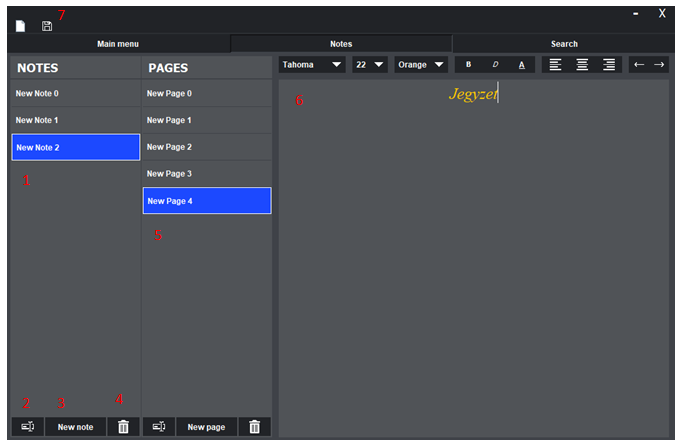
\includegraphics[scale=0.7]{images/doc_1.png}
	\caption{Jegyzetek menü használat közben.}
	\label{fig:menu_notes_2}
\end{figure}

\vspace{5pt} \noindent \textbf{1}-es panel a jegyzetek panelje, itt találhatóak egymás alá beszúrva a különböző jegyzetek. Az éppen kijelölt jegyzet kék színű, kattintással tudunk új jegyzetet kiválasztani, valamint ha a panelen belül az üres részre kattintunk, akkor mindig az utolsó jegyzetet fogja kijelölni.
\newline \\ Található a panelen 3 gomb. 
\vspace{5pt} \\ \textbf{2}-es gomb az éppen kijelölt jegyzet átnevezésére szolgál, egy felugró modális ablakba a beírt szövegre nevezhetjük át a kijelölt elemet, vagy megszakíthatjuk az egész folyamatot. (lásd 5.2 ábra)

\begin{figure}[h]
	\centering
	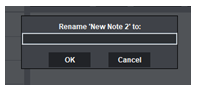
\includegraphics[scale=0.7]{images/doc_2.png}
	\caption{Átnevezésre szolgáló modális ablak.}
	\label{fig:menu_notes_rename}
\end{figure}

\vspace{5pt} \noindent \textbf{3}-mas gombbal új jegyzetet adunk a meglévő jegyzet listához. Alapértelmezett neve a jegyzeteknek ’New Note [sorszám]’.
\vspace{5pt} \\ \textbf{4}-es gombbal az éppen kijelölt jegyzetet törölhetjük, vagy szakíthatjuk meg ezt a folyamatot egy felugró modális ablak segítségével. (lásd 5.3 ábra)

\begin{figure}[h]
	\centering
	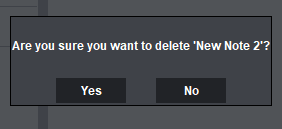
\includegraphics[scale=0.7]{images/doc_3.png}
	\caption{Törlésre szolgáló modális ablak.}
	\label{fig:menu_notes_delete}
\end{figure}

\vspace{5pt} \noindent \textbf{5}-ös panel a lapok panelje. Minden jegyzetnek külön lapjai lehetnek. A panel egyéb funkciói és kezelése teljesen megegyezik az előbb bemutatott jegyzetek menüével.
\vspace{5pt} \\ Ahogy kattintással váltogatunk a jegyzetek között, úgy frissül a lapok menü is, tehát ahogy a beszúrt képen látszik, a ’New Note 2’ jegyzetnek 5 lapja van. Ha átkattintanánk a ’New Note 1’-re, akkor a lapok listája üres lenne, mivel még nem hoztunk létre lapot az adott jegyzethez. Alapvetően jegyzet váltáskor nem jelölődik ki egy lap sem. 
\vspace{10pt} \\ \textbf{6}-os szövegdoboz felületen az éppen kijelölt lap tartalma jelenik meg. A felület mindig frissül, ha új lapra kattintunk, valamint ha nincs egy lap sem kijelölve, akkor üres lesz.
\\A szövegdoboz felett gombok találhatók, amik a szöveg szerkesztésére használhatóak.
\\Balról  jobbra haladva a gombok: 
\vspace{5pt} \\-Szöveg stílus váltás: alapértelmezett Tahoma. Csak a kijelölt szövegrész stílusa fog megváltozni!
\vspace{5pt} \\-Szöveg méret váltás: alapértelmezett 8-as méret. Csak a kijelölt szövegrész mérete fog megváltozni!
\vspace{5pt} \\-Szöveg szín váltás: alapértelmezett fekete szín. Csak a kijelölt szövegrész színe fog megváltozni!
\vspace{5pt} \\-Félkövér betű: kijelölt szövegrész félkövérré alakítása.
\\Gyorsbillentyű: Ctrl + B
\vspace{5pt} \\-Dőlt betű: kijelölt szövegrész dőltté változtatása.
\\Gyorsbillentyű: Ctrl + I
\vspace{5pt} \\-Aláhúzás: kijelölt szövegrész aláhúzása.
\\Gyorsbillentyű: Ctrl + U
\vspace{5pt} \\-Balra, középre, jobbra sorolás: kijelölt szövegrész adott irányba sorolása. Egy sor esetén a szöveg csak egy irányba sorolható.
\\Gyorsbillentyű: Ctrl + Q, Ctrl+E, Ctrl+R
\vspace{5pt} \\-Undo gomb: A szövegdoboz utolsó változtatását visszavonja. Fontos, hogy csak a szövegdobozon működik, note vagy page törlésre, átnevezésre, stb… nem!
\\Gyorsbillentyű: Ctrl + Z
\vspace{5pt} \\-Redo gomb: Az undo gomb ellentéte. Fontos, hogy csak a szövegdobozon működik, note vagy page törlésre, átnevezésre, stb… nem!
\\Gyorsbillentyű: Ctrl + Y

\vspace{5pt} \noindent \textbf{7}-jelzett gomb a mentés gomb. Gyorsbillentyű: Ctrl + S. Fontos, hogy minden egyes alkalommal megnyomni, amikor egy lap tartalmán változtatunk, mert így kerülnek a módosítások mentésre. 
\vspace{5pt} \\Ha nem használjuk, és véletlenül átlépünk egy másik lapra, akkor az összes eddig bevitt információ elveszlik. Szerencsére az Undo gomb használatával visszahozható az elveszett információ, ha ez valamilyen oknál fogva nem működne, akkor a bevitt adatok ténylegesen elvesztek.
\subsection{!!!!!!!!!!!!!Mentést meg kell változtatni, a mentés csak az adatbázisba való mentésre vonatkozzon!}



\newpage \subsection{Kereső menü}

\begin{figure}[h]
	\centering
	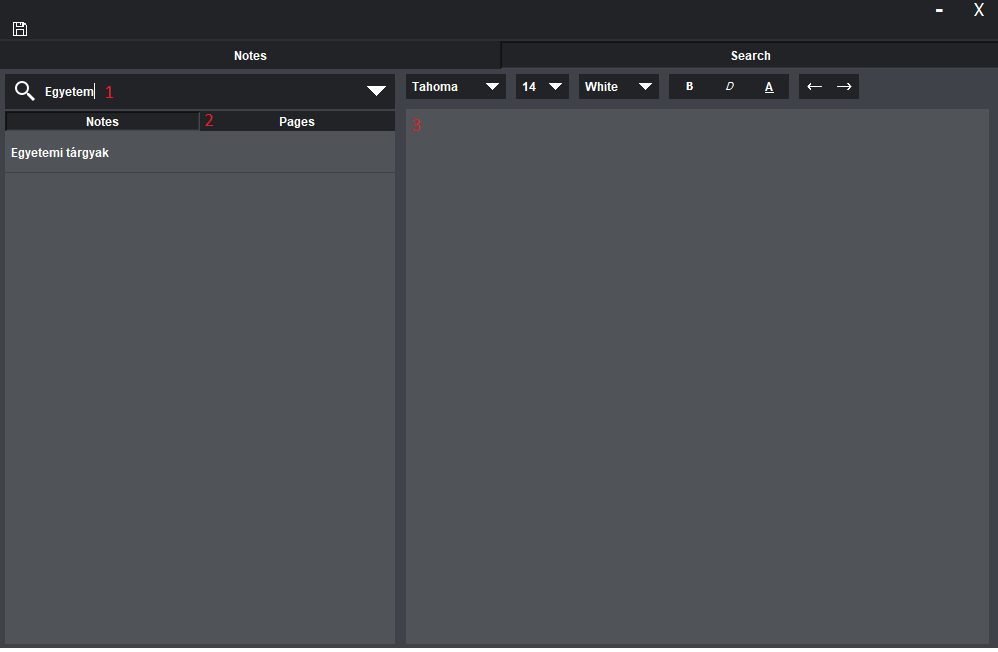
\includegraphics[scale=0.7]{images/doc_4.png}
	\caption{Kereső menü működés közben.}
	\label{fig:menu_search}
\end{figure}

\vspace{5pt} \noindent \textbf{1}-essel jelölt elem a ’search bar’ (kereső sor). Jegyzetek, lapok és lapok tartalma között keres. Ha jegyzet neve, lap neve, vagy lap tartalma tartalmazza a beírt kifejezést, akkor lesz találat. 
\vspace{5pt} \\Hogy a keresés könnyebb legyen, üres search bar-ba való kattintáskor az összes jegyzet és lap neve megjelenik egy listába. Ahogy a keresendő szöveget írjuk be a lista annak megfelelően fog változni. 

\begin{figure}[h]
	\centering
	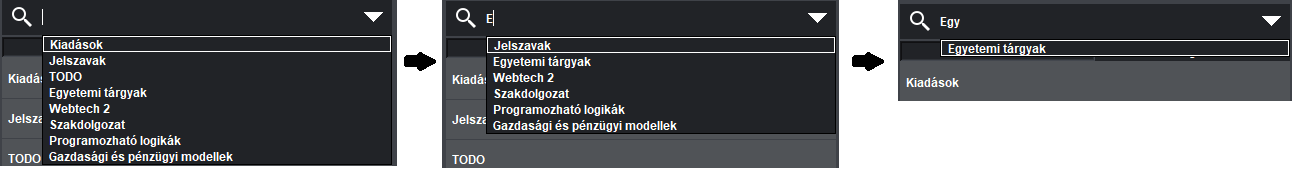
\includegraphics[scale=0.7]{images/doc_5.png}
	\caption{Keresési folyamat szemléltetése.}
	\label{fig:menu_search_searchBar}
\end{figure}
	
\vspace{5pt} \noindent Ha nincs egyezés, a lista eltűnik, nem jelenít meg egyetlen elemet sem.
\vspace{5pt} \\Ha az egyező szöveg egy adott lap tartalmán belül található, tehát nem a nevében, akkor is a listában a lap neve fog szerepelni.
\vspace{5pt} \\A beírt szövegre keresni kijelölés után \underline{csak} a nagyítóra való kattintással lehetséges.
	
	
\vspace{5pt} \noindent \textbf{2}-essel jelölt elem a note és page keresési találatok listája.
\vspace{5pt} \\Alapvetően, hogyha futtatáskor először lépünk be ebbe a menübe egyik sem lesz kijelölve, viszont az első keresés után a jegyzetek listáját fogja megjeleníteni. Hogyha a page-re kattintunk, akkor a talált lapokat fogja megjeleníteni, így tudunk váltani a talált jegyzetek és lapok, illetve lapok tartalma között.
\vspace{5pt} \\Ha a jegyzet találatok között az egyikre rákattintunk, akkor visszakerülünk a Notes Menu-be, hogy meg tudjuk tekinteni az adott jegyzet lapjait, átnevezni vagy törölni tudjunk.
\vspace{5pt} \\Ha a lap találatok között az egyikre kattintunk, akkor nem kerülünk vissza a Notes Menu-be. Az adott lap tartalmát tudjuk szerkeszteni és megtekinteni egy Notes Menu-höz hasonló szövegdobozban \textbf{(3.elem)}. Ennek funkciói teljesen megegyeznek az említett szövegdobozéval és menteni is a ctrl+s-el kell a változtatásokat, vagy a mentés ikonra kattintva.
\vspace{5pt} \\Ha esetleg átnevezni vagy törölni szeretnénk az adott lapot, a Notes Menu-ben tehetjük ezt meg.

		






\subsection{Adattárolás}

Az adatok felhőalapú adatbázisban kerülnek tárolásra, így megoldva a szinkronizáció problémáját. Egy hátránya van ennek, ahogy az adatbázisok leírásánál említettem, ha nincs internetkapcsolat, akkor nem működik a program. Tehát az internetelérés a megfelelő működés szempontjából létfontosságú.
\vspace{5pt} \\Az \textbf{!!!!!!!!!!!XY!!!!!!!!!!!!} adatbázis használata mögött semmi konkrét indoklás nincs, nem nyújt semmi extra funkciót, amiért ezt a szolgáltatót választottam másik helyett.

\subsection{Titkosítás és kulcskezelés}

Az adatok védelmére az AES titkosítási algoritmust használtam, főként a tesztekből megállapított tulajdonságai miatt. Mivel az alkalmazást én fogom használni a későbbiekben, nem nagyobb célközönség felé irányul, ezért egy aszimmetrikus titkosítási algoritmus használatát végképp nem látom szükségesnek.
\\A titkosítási folyamat és a kulcskezelés is alkalmazás szintjén történik. Nagy valószínűséggel adatbázis szintjén is meg lehetett volna ezt oldani, ez igazából az adatbázis szolgáltató iránti bizalmon alapszik, hogy az ember megbízik-e a szolgáltató kulcskezelési és titkosítási módszereiben.

\subsection{!!!!VALAMILYEN RÉSZLETES FORRÁSKÓD KÉNE IDE + KEYMANAGEMENT LEÍRÁS, INDOKLÁS!!!!}



\newpage
A fejezetben be kell mutatni, hogy az elkészült alkalmazás hogyan használható.
(Az, hogy hogyan kell, hogy működjön, és hogy hogy lett elkészítve, az előző fejezetekben már megtörtént.)

Jellemzően az alábbi dolgok kerülhetnek ide.
\begin{itemize}
\item Tesztfuttatások. Le lehet írni a futási időket, memória és tárigényt.
\item Felhasználói kézikönyv jellegű leírás. Kifejezetten a végfelhasználó szempontjából lehet azt bemutatni, hogy mit hogy lehet majd használni.
\item Kutatás kapcsán ide főként táblázatok, görbék és egyéb részletes összesítések kerülhetnek.
\end{itemize}
